\documentclass[sigconf]{acmart}
\usepackage{listings}  
\usepackage{xcolor}  
\usepackage{tabulary}
\usepackage{tikz}
\usetikzlibrary{shapes,arrows,positioning,fit,backgrounds}

%% \BibTeX command to typeset BibTeX logo in the docs
\AtBeginDocument{%
  \providecommand\BibTeX{{%
    Bib\TeX}}}

\begin{document}

\title{Implementing an on-demand data preparation approach}


\author{Ahmed Rezk}
\affiliation{
    \institution{University of Stuttgart}
    \city{Stuttgart}
    \country{Germany}
}
\email{st163697@stud.uni-stuttgart.de}
    
\author{Luke Mayr}
\affiliation{
    \institution{University of Stuttgart}
    \city{Stuttgart}
    \country{Germany}
}
\email{st177937@stud.uni-stuttgart.de}

\author{Metin Arab}
\affiliation{
    \institution{University of Stuttgart}
    \city{Stuttgart}
    \country{Germany}
}
\email{st178931@stud.uni-stuttgart.de}

\author{Tabea Steeb}
\affiliation{
    \institution{University of Stuttgart}
    \city{Stuttgart}
    \country{Germany}
}
\email{st156637@stud.uni-stuttgart.de}

\begin{abstract}
    Data has never been as significant as it is today. 
    It can be acquired virtually at will on any subject.
    Data is digital Oil. Within this digital age, it is crucial for humanity in almost every domain. 
    Additionally, data is not restricted in quantity, meaning limited data can be generated for use.
    Along with this growing demand, the processing of this data must develop to keep up.
    The goal has to be demand-driven data provisioning, i.e., the right data must be available in the right form at the
    right time. 
    Our goal is to develop a demand-driven application for data lakes.
    Therefore, we created a tailorable data preparation zone called BARENTS.
    The users can decide what data is derived how and where.
    The users are not required to understand the background process, only the basic steps.
    We developed a prototype and compared several methods of implementation.
\end{abstract}

\keywords{Data Lake, data preprocessing, ontology, BARENTS, LALO}

\maketitle

\section{Introduction}
The Barents paper is organized as follows: Section 2 discusses the background of Barents and its overall concept. Section 3 discusses our requirement specification for building the prototype BARENTS. Section 4 evaluates ontology editors and whether they can be used for the BARENTS prototype. Section 5 outlines the prototype implementation and the structure of the frontend and backend system. In section 6 we evaluate our requirement specification from section 3. Finally, in Section 7 we conclude and summarize our work.

\section{Background}
\label{background}

    We want to develop our Editor with the concept BARENTS. In this section we will have a closer look at BARENTS and introduce a scenario, in which our Editor might be of use: testing chocolate samples for nut allergens. This section \ref{background} is mainly based on \cite{barents21} and \cite{barents22}.

    \subsection{Overview BARENTS}
        \label{barents}
        Data can be a valuable resource, but often it has to fit a specific use case (demand-driven data provisioning). 
        With BARENTS, a user can specify how to pre-process data. It is a tailorable data preparation zone for data lakes. 

        In an ontology the user defines the following:
        \begin{itemize}
            \item (data level) the data source
            \item (information level) a transformation (how the data should be processed), which can be:
            \begin{itemize}
                \item filter: eliminate or select data
                \item map: modify data
                \item reduce: aggregate data (a set of data gets one output value)
                \item other procedure: a user-defined function
            \end{itemize}
            \item (knowledge level) the data sink, where the results are stored
        \end{itemize}
        According to the created ontology the data then is automatically processed and delivered. 

        \begin{figure}[h]
            \noindent
            \centering
            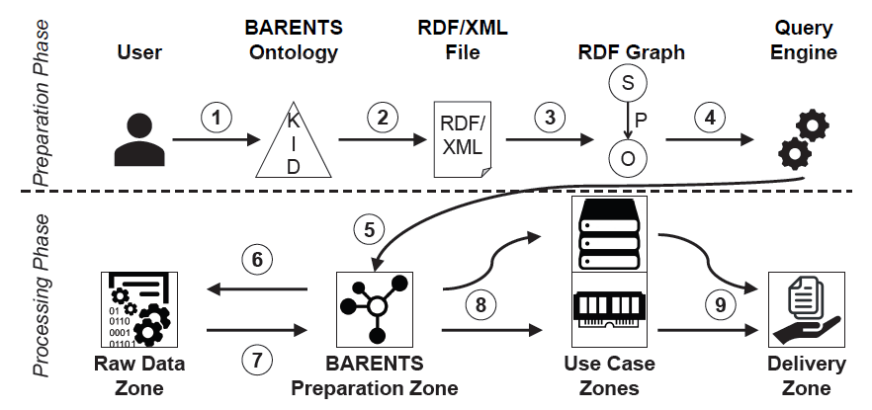
\includegraphics[width = \columnwidth]{BARENTS_operationProcess.png}
            \Description{operation process of BARENTS}
            \caption{operation process of BARENTS}
            \label{operationProcess}
        \end{figure}

        In figure \ref{operationProcess} we can see how BARENTS operates: 

        \begin{enumerate}
            \item the user models the pre-processing steps for his use case (as an ontology), e.g. with a graphical editor.
            \item this ontology is saved as a RDF/XML file
            \item 5. RDF/XML file is processed
            \item all data sources (listed in the ontology) are retrieved from the "raw data zone"
            \item the pre-processing steps are applied on the data
            \item the pre-processed data is forwarded to the (in the ontology indicated) "use case zone"
            \item user can access this data in the "delivery zone"
        \end{enumerate}

    \subsection{Use case scenario: nut allergens in chocolate samples}

        On food packaging, it is important to write the correct allergy information, as food allergies can trigger severe allergic shocks. So for our use case scenario, chocolate is tested whether it contains nut allergens.

        Chocolate samples are tested with a mass spectrometer, if they contain "allergenic peptides", i.e. fragments of proteins. 
        The thereby created raw data is cross-checked against a protein sequence database to figure out if the sample contains hazelnut or walnut peptides. Sample, that contain nut allergens, are marked. 

        The food chemist, (the "domain expert"), now wants to filter out unmarked chocolate samples, so he can use the marked samples (with nuts) for further analysis.
        \begin{figure} [H]
            \noindent
            \centering
            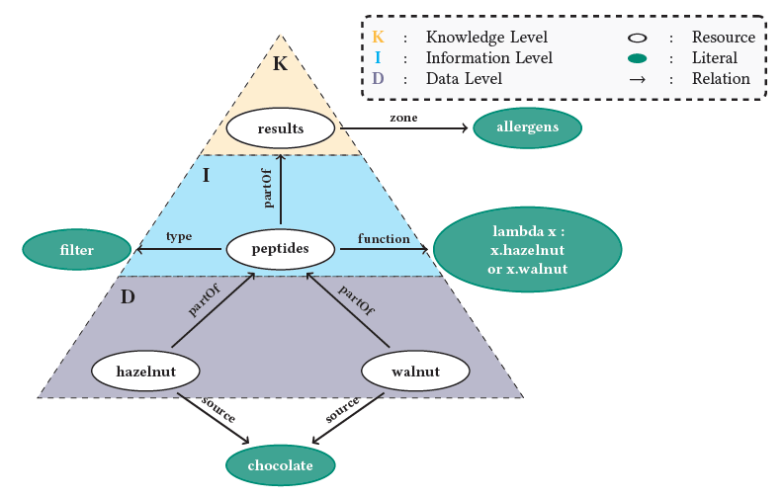
\includegraphics[width = \linewidth]{BARENTS_ontologyExample.png}
            \Description{graphical depiction of the BARENTS ontology for the chocolate example}
            \caption{graphical depiction of the BARENTS ontology for the chocolate example}
            \label{ontologyExample}
        \end{figure}

        For that purpose the food chemist can create an ontology in BARENTS. In figure \ref{ontologyExample} we can see that ontology depicted.

        In the data level the information about hazelnut and walnut in the database chocolate get extracted and loaded into a new table "peptides". 
        In the information level the chocolate samples that are marked as containing hazelnuts or walnuts are filtered out. 
        On the knowledge level the results are then stored in the use case zone "allergens". 

        A domain expert with no knowledge about databases should still be able to work with data, which is why we want to develop an easy-to-use editor for BARENTS.

        In figure \ref{RDFExample} we can see how the from BARENTS automatically created RDF/XML file might look like with the chocolate example.
        \begin{figure} [H]
            \noindent
            \centering
            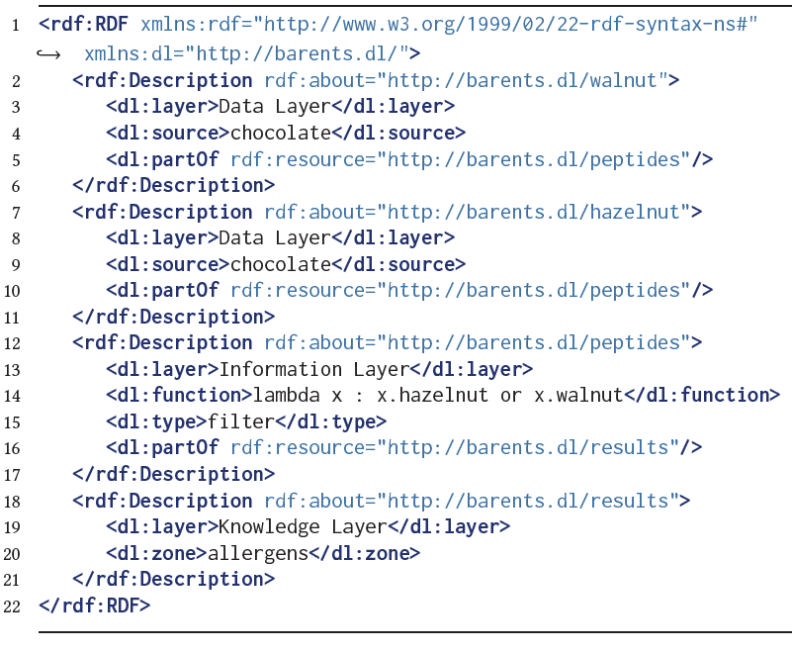
\includegraphics[width = \columnwidth]{BARENTS_RDFExample.png}
            \Description{from the chocolate example created RDF/XML file}
            \caption{from the chocolate example created RDF/XML file}
            \label{RDFExample}
        \end{figure}



\section{Requirement Specification}
    \begin{enumerate}
        \item[(R1)] Our goal is an Easy-to-use GUI for domain experts, with which they can create ontologies.
        %% TODO: hier statt \cite{barents21} die Stelle im Kapitel Barents angeben
        \item[(R2)]  minimum one of the Transformations I,II or III as defined in \cite{barents21} (namely filter, map or reduce operator) is functioning.
        \item[(R3)] Created ontologies can be saved.
        \item[(R4)] Has a data-processing-engine, which processes data according to the ontology.
        \item[(R5)] Our prototype should be functioning with at least one database type. We chose relational databases, since we are most familiar with that.
    \end{enumerate}

    %% dieses Kapitel optional


\section{Implementation}
    \subsection{Discussion on own implementation vs. existing tools}
        \subsubsection{OWLGrEd}
            OWLGrEd \cite{owlgred} is a free graphical editor for OWL ontologies in UML style \cite{owlgredW3}. 
            It has classes and different connections, including (directed) associations. 
            The classes we could modify for the data source and data sink and the association for the data transformations. 
            However, this modification would be very time-consuming: classes somehow need to connect to the data source or sink, connections should have different types according to the transformations (filter, map, reduce), and the whole toolbar should be slimmed down to only the necessary tools. 
            An example ontology create in OWLGrEd is given in \autoref{OwlGrEd-image}.

            \begin{figure}[h]
                \centering
                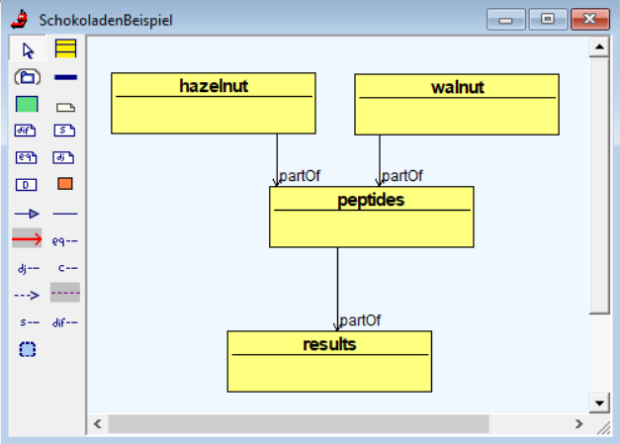
\includegraphics[width = \columnwidth]{Owlgred.png}
                \Description[Example instance of the BARENTS ontology create with OWLGrEd]{Shown here is the OWLGrEd Editor in which an instance of the BARENTS ontology was created}
                \caption{Example instance of the BARENTS ontology created with OWLGrEd}
                \label{OwlGrEd-image}
            \end{figure}


            OWLGrEd already has a function to save the created ontology as a RDF/XML file (*.owl). But here as well would we need to modify a lot such that the RDF/XML file suits the BARENTS model. 

            The code is written in Lua (which we are not familiar with) and is difficult to understand (lots of code, with unclear structure, often not or in different languages commented). 

            All in all it would be much work to alter the editor to our needs.

        \subsubsection{WebVowl}
            WebVowl creates and edits ontologies, using a GUI, which simplifies the ontology modeling process\cite{lohmann2015webvowl}.
            It has no drag-and-drop functionality, it, instead,  creates components on-double-click.
            Its both possesses import and export functions.
            However, it can only export TTL-files.
            Yet it is fixable due to the possibility of auto-converting TTL- to XML-/RDF-files using the tool Apache Jena.

            Our problem with WebVowl was that there is a lack of information about the structure of the code.
            This lack of context made it really difficult, for us, to edit or extend the source code.
        \subsubsection{Protégé}
            Protégé is an open Source ontology editor\cite{musen2015protege}. One if it main core features that you can extend it functionality by building your own plugins. However after carefully examining and using Protégé, we determine that the UI is complex, as requires us to watch multiple tutorials just to navigate and use it effectively, which goes against our easy-to-use requirement (R1).
            Moreover, the process of developing Protégé plugin is not clear and the some of the available information became outdated or is no longer accessible. 
        \subsubsection{CoModIDE}
            CoModIDE is a plugin for Protégé, that allows users to create and edit ontologies graphically\cite{shimizu2019comodide}. With its drag-and-drop functions, creating and editing ontologies is relatively easy. However, the Problem with CoModIDE is that it models RDF graphs in a very general way, which means that not all available features are easily applicable to BARENTS and are not tailored to domain experts.  
        \subsubsection{implementing ourselves}
            The last consideration we made was implementing the prototype ourselves, from the ground up. 
            This approach is much more structured, as it allows us to only implement necessary features and model the applications architecture for the BARENTS ontology specifically. 
            On the flipside this would lead to a larger workload. 

            In order to accurately assess the feasibility of such an implementation, we created a total of three iterative mockups. 

    \subsection{evaluation}
        Finally, we compare the various editors previously discussed (pictured in \autoref{Editor-table}).

        \begin{table} [h]
            \centering
            \begin{tabulary} {\paperwidth} {p{1,5cm}|p{2,5cm}|p{1,3cm}|p{2,5cm}}
                Editor & design & language, Tools & Problems \\ \hline
                OwlGrEd & UML-style classes and connections & java & unclear and complex Code, timeconsuming to adapt \\ \hline
                WebVowl & GUI to draw graph&JavaScript& exports only TTL, code structure unclear \\ \hline
                Protégé & extendable via plugins & Java& Complex UI; not enough information to develop ow plug in\\ \hline
                CoModIDE & GUI with drag and drop feature to draw RDF graph & Java&too general for Barents, not for domain experts \\ \hline
            \end{tabulary}
            \caption{Comparison of Ontology Editors discussed}
            \label{Editor-table}
        \end{table}


\section{Prototyping}
    \subsection{Scope of the Prototype}
        Our prototype is supposed to be a proof of concept for the utility of a GUI that allows users to create a configuration file following the BARENTS specifications. 
        It is worth noting that BARENTS was conceived for the purpose of data provisioning in data lakes.
        Our prototype will only support data provisioning in select relational databases. 
        This allows for both the desired proof of concept, while keeping the scale much for feasible.

    \subsection{Data Access and the Expanded BARENTS Ontology}
        In the BARENTS ontology as described by Stach et al.~\cite{barents21} data features are represented by resources in the ontology.
        This by itself doesn't allow for data access, as metadata such as access credentials and its storage location are missing.  
        The BARENTS zone architecture by Stach et al.~\cite{barents21} contains a Management Zone which provides this information. 
        Later that information is modeled by additional literals in the BARENTS ontology.

        Considering the scope of this project, we opted to omit the Management Zone.
        As such there is no data catalogue for our prototype to reference. 
        Therefore we require the user to provide both a database location, as well as a table within that database. 
        This information is the modeled as two seperate literals.

        Finally, we provide an instance of this expanded BARENTS ontology in \autoref{BARENTS-instance-pyramid}.
        \begin{figure}[h]
            \centering
            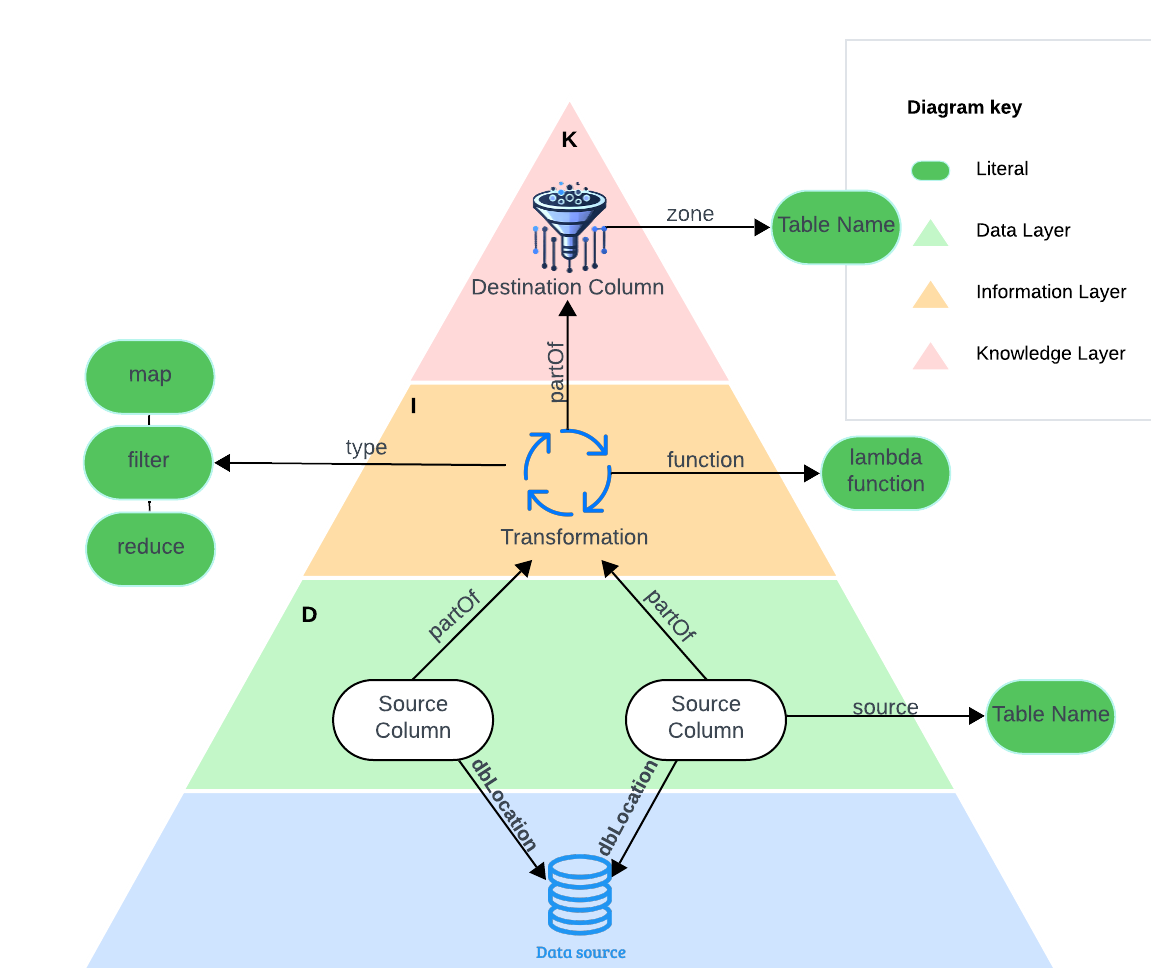
\includegraphics[width = \columnwidth]{Pyramid Chart - Page 1.png}
            \Description{Instance of the expanded BARENTS ontology}
            \caption{Instance of the expanded BARENTS ontology}
            \label{BARENTS-instance-pyramid}
        \end{figure}


\subsection{Frontend design}
\begin{figure}[h]
    \centering
    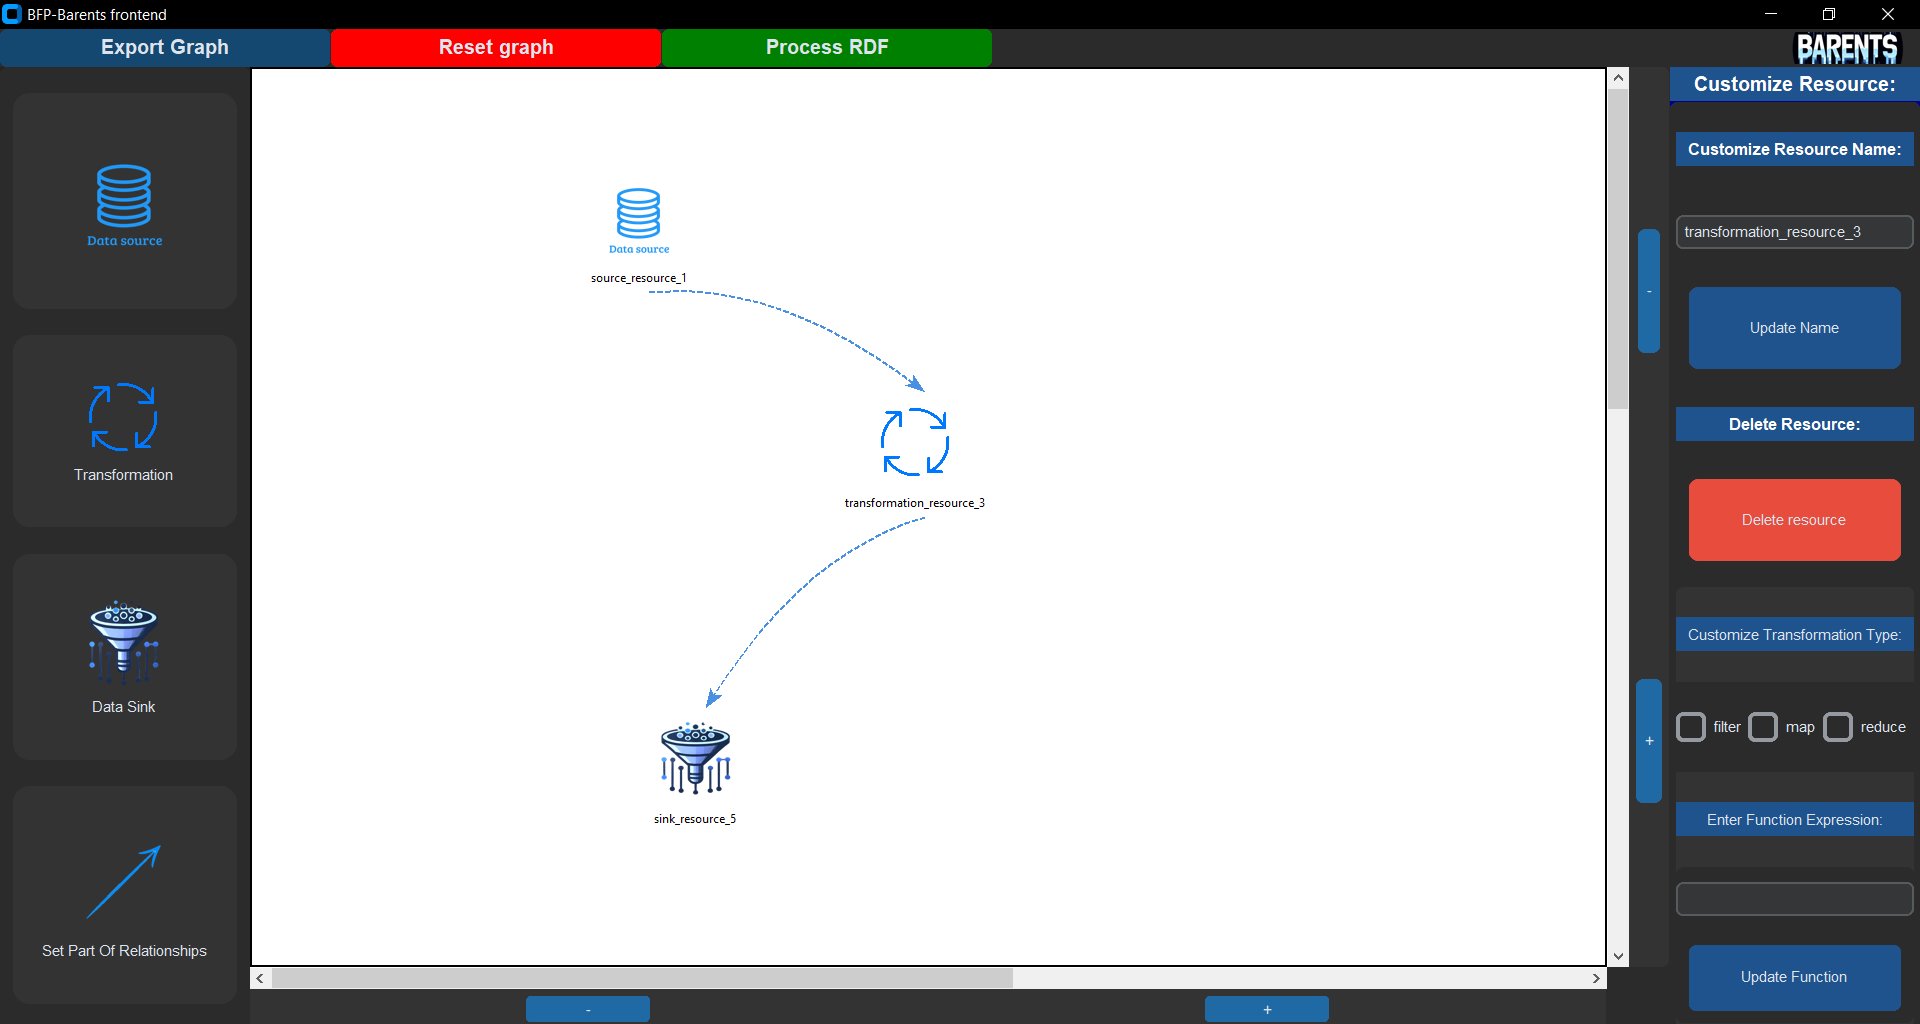
\includegraphics[width = \columnwidth]{GUI_interface.PNG} 
    \Description{The prototype of the BARENTS Editor}
    \caption{The prototype of the BARENTS Editor}
    \label{BARENTS-editor} 
\end{figure}
The User Interface for the Barents project(pictured in\autoref{BARENTS-editor})
is built on CustomTkinter\cite{customtkinter}.It is a Python library that provides a modern look for the user interface. As  our Backend also uses Python,we chose to use CustomTkinter, allowing us to have one
programming language instead of managing multiple programming languages simultaneously. 
Our UI adopts a minimalistic design. 
The layout is divided into a canvas, making up most of the screen space, along with a left, right and top bar. 
Our goal was to minimize the number of buttons and give them a reasonable size to ensure simplicity and a good user experience. 

The left bar contains only four buttons, which are the buttons for the addition of source, transformation, sink and part of Relationship arrows. Each button is
represented with a corresponding symbol, making it easier for
the user to understand and differentiate between the nodes in the
canvas.

By selecting the node, a corresponding right-side panel opens,
giving the user specific textboxes with clear labels indicating what
information is required for the node, to meet the ontology requirements. 

Finally, the user can export the graph in formats, such as XML, ttl, jasonld, nt and n3 and process RDF/XML files not created by our UI, as long they follow the Barents namespaces.

\begin{figure}
    \noindent
    \centering
    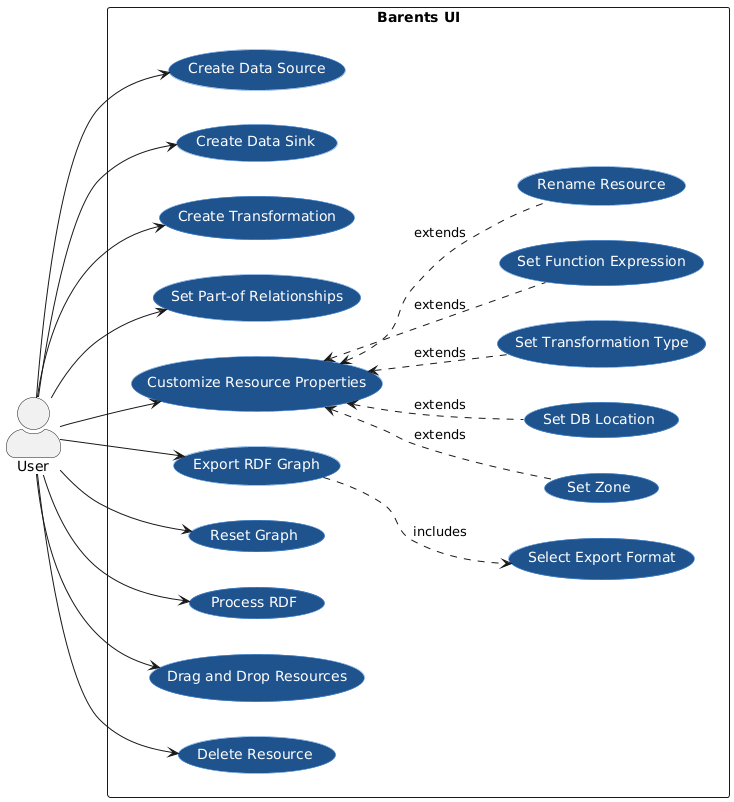
\includegraphics[width = \columnwidth]{USE-Case Diagaramm.png}
    \Description{Use-case diagram showing users possible interactions with the Braents UI}
    \caption{Use-case diagram showing users possible interactions with the Braents UI}
    \label{FrontendDesign}
\end{figure}

\subsection{Backend}
This Section discusses the overall structure and design of the backend system. 
\subsubsection{Libraries}
Our backend system uses SQLite3\cite{python_sqlite3} and rdflib\cite{rdflib} libraries, which play an integral part in our backend functionality. As our frontend system exports our ontology RDF/XML files, we use RDFLib to create the graph internally in the system and parse through it. This allows us to extract relevant information from the ontology graph. For example, Database location, that can later establish a connection to it through SQLite. For now, our backend system supports local  SQlite Databases, that can manipulate and transform relational data.
\subsubsection{Parsing Algorithm}
One of the key challenges in developing the backend system is parsing through the RDF graph and extracting only relevant information related to the transformation for SQlite3. As we tried to cover the use case, if the user created a graph with multiple transformations, then each transformation has to be executed separately and use only data Sources and Data Sink, that it is only connected to it through the partOf relationship. The following Figure  \ref{rdf_parsing} gives a brief overview of the parsing of the RDF graph. 
\begin{figure}[h]
\centering
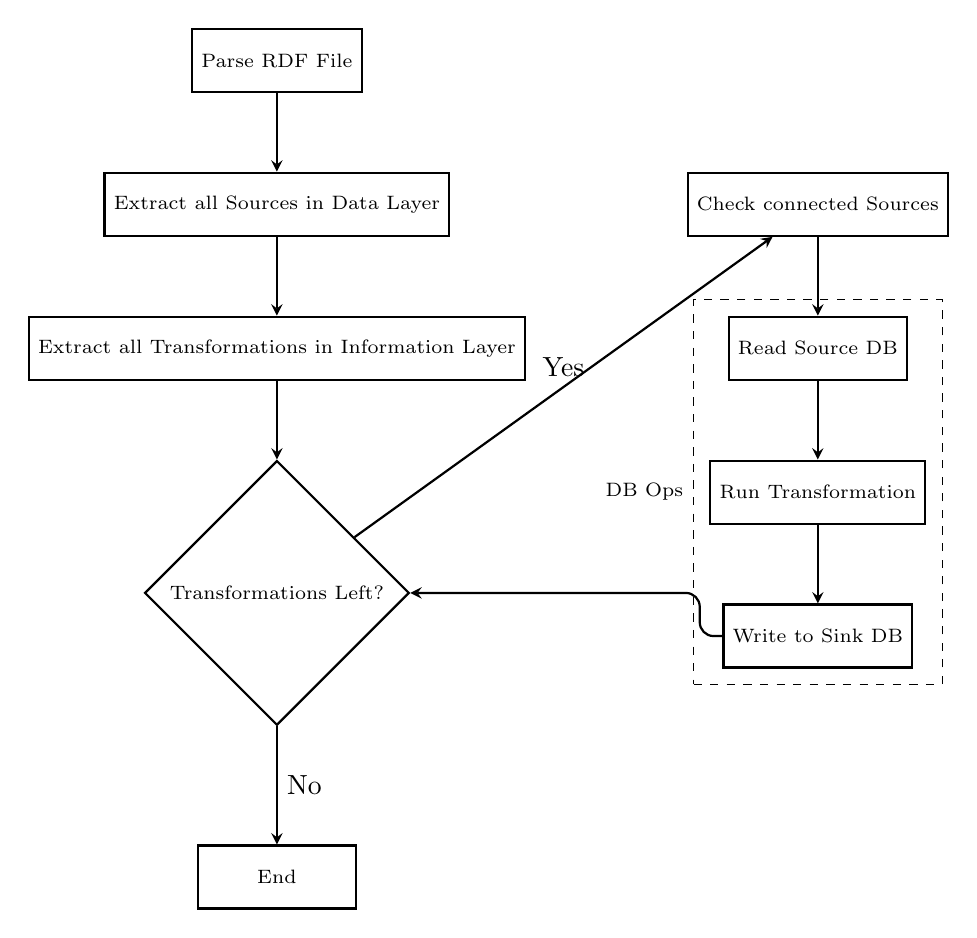
\begin{tikzpicture}[
    auto,
    node distance=1cm,
    thick,
    process/.style={
        rectangle,
        draw,
        text centered,
        minimum height=0.8cm,
        minimum width=2cm,
        font=\scriptsize
    },
    decision/.style={
        diamond,
        draw,
        text centered,
        minimum height=0.8cm,
        minimum width=2.5cm,
        font=\scriptsize
    },
    arrow/.style={->, >=stealth, rounded corners=5pt}
]
    
    \node[process] (parse) {Parse RDF File};
    \node[process, below=of parse] (sources) {Extract all Sources in Data Layer};
    \node[process, below=of sources] (trans) {Extract all Transformations in Information Layer};
    \node[decision, below=of trans] (check) {Transformations Left?};
    \node[process, below=1.5cm of check] (end) {End};
    
    
    \node[process, right=3cm of sources] (required) {Check connected Sources};
    \node[process, below=of required] (read) {Read Source DB};
    \node[process, below=of read] (run) {Run Transformation};
   \node[process, below=of run] (write) {Write to Sink DB};
    
    
    \draw[arrow] (parse) -- (sources);
    \draw[arrow] (sources) -- (trans);
    \draw[arrow] (trans) -- (check);
    \draw[arrow] (check) -- node[above] {Yes} (required);
    \draw[arrow] (check) -- node[right] {No} (end);
    \draw[arrow] (required) -- (read);
    \draw[arrow] (read) -- (run);
    \draw[arrow] (run) -- (write);
    \draw[arrow] (write) -- ++(-1.5,0) |- (check);
    
    
    \begin{pgfonlayer}{background}
        \node[draw=black,dashed,fit=(read)(run)(write),
        inner sep=0.2cm,label=left:{\scriptsize DB Ops}] {};
    \end{pgfonlayer}
\end{tikzpicture}
\Description{RDF Parsing Algorithm}
\caption{RDF Parsing Algorithm}
\label{rdf_parsing}
\end{figure}
\subsubsection{Filter Operation}
Before calling any of the transformation operation,
a run transformation function shown in Listing \ref{listing} is called,
and queries the RDF graph to identify the transformation type in the Information layer.
In our backend, we  only implemented a dynamic filter operation that leverages Python lambda functions, giving the user a wide range of filtering criteria.

We start the filtering operation by extracting relevant MetaData. We identify with the help of rdflib Sink Table(target Table), its corresponding Database, and the user-specified lambda expression. As a transformation can have multiple Data Sources, we identify the ones connected to the transformation and store them in a set. We later on establish connections with the help of sqlite3 library in Python to all the Databases that we extracted.
\lstset{
    language=Python,
    basicstyle=\ttfamily\footnotesize,  % Smaller font size
    keywordstyle=\color{blue},
    commentstyle=\color{gray},
    stringstyle=\color{red},
    numbers=left,
    numberstyle=\tiny\color{gray},
    stepnumber=1,
    numbersep=5pt,
    backgroundcolor=\color{white!20},
    showspaces=false,
    showstringspaces=false,
    frame=single,
    breaklines=true,  % Enable line breaking
    breakatwhitespace=true,
    captionpos=b,
    xleftmargin=0.5cm,  % Adjust left margin
    xrightmargin=0.5cm  % Adjust right margin
}


\begin{lstlisting}[caption={Transformation function}, label={listing}]
    def run_transformation(transformation, sources):
    transformation_type = rdf_graph.value(transformation, dl.type).strip()
    match transformation_type:
        case "filter":
            filter(transformation, sources)
        case "map":
            map(transformation,sources)#TODO
        case "reduce":
            reduce(transformation,sources)#TODO
                        
\end{lstlisting}

As we store the relevant Data Sources in a set, we iterate through each one and execute an SQL command to select all rows from the table in the source database and apply the filter function, which is the lambda function to every row of the table. If the function returns True the row is kept and inserted into the designated sink table, through an SQL command.

\begin{figure}[h]
  \centering
  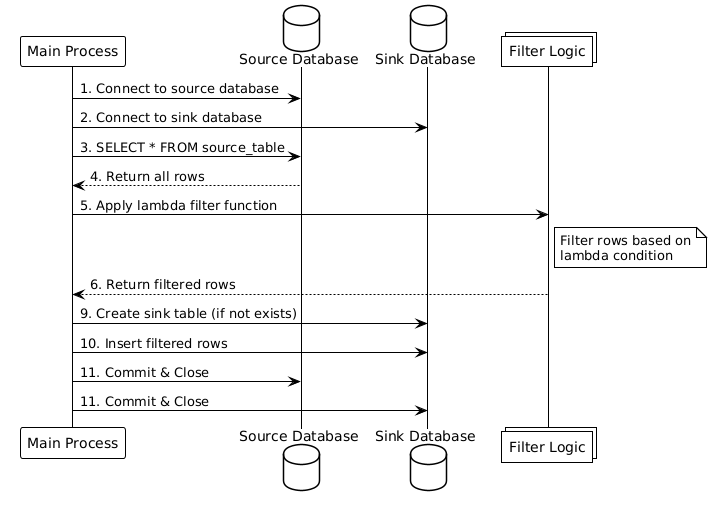
\includegraphics[width=1\linewidth]{Sequence_diagramm.png}
  \Description{Sequence diagram illustrating the filter operation}
  \caption{Sequence diagram illustrating the filter operation}
  \label{sequence}
\end{figure}

\section{Evaluation - Requirements Fulfillment}
    In this section, we evaluate our project towards or previously set requirements in Section 3.
    For the easy-to-use requirement R1, we kept our UI design minimalistic, used the least amount of buttons, and only kept features that are relevant to the creation of Ontology. These decisions were taken based on the review of other ontology editors that were hard to understand or had unnecessary features for our project, that would overcomplicate things for domain experts.
    Moreover, the R3 requirement is fulfilled, as the user can save the created ontologies graphs in various formats, giving flexibility for future Developers to design their own Data Processing engine, that does not only have work RDF/XML files

    We have built a small data-processing-engine, that can process data according to the ontology, and utilizes SQLite to transform relational databases. The Transformation I, namely filter has been implemented in our engine, however, the full functionality of the filter operation is limited by....(name limitations). However, we can say that requirements R4 create a data-processing engine, R5 prototype works with at least one relational database, and R2 implementing Transformation I, are partially fulfilled.

\section{Conclusion}
    Virtual data will only increase in importance in the future. 
    In order to get the most profit out of it, we need to manage it efficiently.
    We have developed a tailorable data preparation zone for data lakes called BARENTS that for demand-driven data management.
    We firstly described the concept of BARNETS and explained what makes it so important.
    Then we explained how we implemented our application and why we decided to implement ourselves, without plugins.
    BARENTS performs efficiently, and fulfills all criteria for good data preparation.
    Our implementation has been a succes and we look forward to further plugins or extensions of our appliction.

%% The next two lines define the bibliography style to be used, and
%% the bibliography file.
\bibliographystyle{ACM-Reference-Format}
\bibliography{references}


\end{document}
\endinput
